%% LyX 2.3.7 created this file.  For more info, see http://www.lyx.org/.
%% Do not edit unless you really know what you are doing.
\documentclass[12pt,english]{article}
\usepackage[T1]{fontenc}
\usepackage[latin9]{inputenc}
\usepackage{geometry}
\geometry{verbose,tmargin=1cm,bmargin=2cm,lmargin=3cm,rmargin=3cm,headheight=3cm,headsep=3cm,footskip=1.2cm}
\usepackage{array}
\usepackage{float}
\usepackage{multirow}
\usepackage{amsmath}
\usepackage{amsthm}
\usepackage{amssymb}
\usepackage{graphicx}
\usepackage{setspace}

\makeatletter

%%%%%%%%%%%%%%%%%%%%%%%%%%%%%% LyX specific LaTeX commands.
%% Because html converters don't know tabularnewline
\providecommand{\tabularnewline}{\\}

%%%%%%%%%%%%%%%%%%%%%%%%%%%%%% Textclass specific LaTeX commands.
\theoremstyle{plain}
    \ifx\thechapter\undefined
      \newtheorem{assumption}{\protect\assumptionname}
    \else
      \newtheorem{assumption}{\protect\assumptionname}[chapter]
    \fi

%%%%%%%%%%%%%%%%%%%%%%%%%%%%%% User specified LaTeX commands.
\usepackage[T1]{fontenc}
\usepackage{tgtermes}
%\usepackage{librebaskerville}
\usepackage{mathtools}
\usepackage{amsmath}
\usepackage{xparse}
\usepackage{lscape}
\usepackage[section]{placeins}
\usepackage{apacite}
\usepackage{etoolbox}
\patchcmd{\thebibliography}{\section*{\refname}}{}{}{}


\usepackage{titlesec}
\usepackage{bbm}


\usepackage{longtable}
\usepackage{booktabs}
\usepackage{sectsty}
\usepackage[toc,page]{appendix}

\tolerance=1
\emergencystretch=\maxdimen
\hyphenpenalty=10000
\hbadness=10000

\usepackage{color, colortbl}
\usepackage[first=0,last=9]{lcg}
\usepackage[left,modulo]{lineno}


\usepackage{soul}
\usepackage{color}

\usepackage[absolute]{textpos}


\newcommand{\hlc}[1]{{\sethlcolor{LightCyan}\hl{#1}}}
\newcommand{\hly}[1]{{\sethlcolor{LightYellow}\hl{#1}}}
\newcommand{\hlw}[1]{{\sethlcolor{White}\hl{#1}}}
\newcommand{\hlg}[1]{{\sethlcolor{LightGreen}\hl{#1}}}

\definecolor{Gray}{gray}{0.9}
\definecolor{LightCyan}{rgb}{0.88,1,1}
\definecolor{LightYellow}{RGB}{255,255,200}
\definecolor{LightGreen}{RGB}{204,255,204}
\definecolor{White}{RGB}{255,255,255}
\newcommand{\ra}{\rand0.\arabic{rand}}


\makeatletter
\@addtoreset{section}{part}
\def\@part[#1]#2{%
    \ifnum \c@secnumdepth >\m@ne
      \refstepcounter{part}%
      \addcontentsline{toc}{part}{\thepart\hspace{1em}#1}%
    \else
      \addcontentsline{toc}{part}{#1}%
    \fi
    {\parindent \z@ \raggedright
     \interlinepenalty \@M
     \normalfont\centering
     \ifnum \c@secnumdepth >\m@ne
       \large\bfseries \partname\nobreakspace\thepart
       \par\nobreak
     \fi
     \huge \bfseries #2%
     \markboth{}{}\par}%
    \nobreak
    \vskip 3ex
    \@afterheading}
\renewcommand\partname{Topic}
\makeatother

\makeatother

\usepackage{babel}
\providecommand{\assumptionname}{Assumption}

\begin{document}
\title{Status Expenditure under Income Inequality}
\maketitle
\begin{abstract}
Status motivations for consumption have generated an immense interest
at a time when social mobility has been relatively stagnant - but
the consequences of inequality on consumption are still poorly understood.
To explain status motivations under environments of income inequality,
the opportunities for mobility are treated as a link between economic
and social goals of the individual while status consumption is viewed
as an investment towards future economic success. The effect of relative
incomes on the agents\textquoteright{} consumption and labour decisions
is then explored in an economy with a dynamic hierarchy of rich and
poor positions that participants are able to move between. With diminishing
returns to wealth utility - which is optimised by participants endowed
with randomly distributed success-determining attributes - the results
indicate that a rise in income inequality provides more incentive
to participate in status competitions. As participants bear costs
for the mobility, the long-term equilibrium conditions suggest two
states - one where both rich and poor strive for status and the other
where only the rich  participate in status competitions.
\end{abstract}

\section{Introduction}

%[The QUESTION]

\noindent

The consumer response to relative income has appealed to economists
since at least as far back as \citeA{VeblenLeisureClass}. While the
post-war improvements in life-standards \cite{HirschSocialLimits,FrankPond}
have renewed an interest in positional concerns, the effects of economic
inequality on status consumption remain unclear. On one hand, the
post-war literature on status competitions attributes higher status
consumption to a fall in income inequalities and improvement in life-standards
\cite{HirschSocialLimits,GalbraithBeyondContentment1994,GalbraithAffluent,roychowdhuryInequalityStatusConsumption2016} 
but on the other hand, empirical studies continue to associate more
status consumption with higher economic inequality \cite{nieftagodien2007blacksconsumption,JinLiInequalityStatusConsumption2011,MazzoccoRuckerStatusConsVicariousIdentification2012,jaikumar2018showoff,ChaiKaus2019}. 

\noindent

The literature in sociology (see \citeA{wegener1992prestigeconcepts}
for a discussion) has argued that one reason why such contradictions
arise is that our attributions to status-differences do not always
reconcile the subjective aspects of status (the effect of status differences
on individual behaviour) with its objective aspects (the observed
reality of status differences). The paper attempts to address this
issue by assuming a specific link between economic and social goals
and thus by allowing status to have an indirect (instrumental) effect
on consumer wealth \cite{ColeMaliathSocialNorms1992,postlewaite1998socialbasisinterdeppreferences}.
Restricting our discussion to social capital investments that increase
the chances for economic mobility (e.g. education, club memberships
etc.), status competitions are viewed as games that provide direct
gains to the participants as probabilistic economic rewards pertaining
to status. 

\noindent

The relationship between economic and social goals of an individual
are delineated using probability functions that determine a promotion
to a richer economic class. The probability of promotion for the participant
is driven both by her social capital investment and a set of fixed
individual attributes. Further, the status of the participant comes
only from her accumulated wealth and is not directly factored into
the utility (an approach similar to \citeA{ColeMaliathSocialNorms1992,postlewaite1998socialbasisinterdeppreferences}
). In the probabilistic game thus defined, the participants compete
both with raw talent and acquired skills (social capital) to get promoted
to (or to maintain) a rich position. More specifically, the winner
of such a game is promoted to a rich position (or maintains her rich
position) by having the maximum total score comprising both of raw-talent
$r_{i}$ (uniformly distributed in a population) and social capital
$s_{i}$ (enhanced with expenditure). The social-capital $s_{i}$
that is enhanced through expenditure is also subject to budget constraints
imposed on the participant.

The game comprises only of two types of participants in the above
view of status - the poor and the rich - so that the investments towards
status (such as club-membership fees, or higher-education) increase
the chances to be promoted to the rich status. The rich participants
in the game or those who benefit with a higher disposable income ($y_{2}$)
solely on grounds of their rich status while the poor participants
are those who receive a disposable income $y_{1}<y_{2}$. Those who
don't participate in the tournament certainly suffer with being poor,
but those who do spend only benefit probabilistically. 

A useful analogy to explain such a competition is that of tennis leagues
or golf tournaments - where rewards are risky but are unlike lotteries
(i.e. more expenditure does not linearly increase one's chance to
win). As with tennis or golf, participants with appropriate raw-talent
and skills may exist naturally in a population but their success also
depends on institutional engagement with other players. More specifically,
there may exist biological characteristics such as strength, dexterity,
height or psychological attributes (resilience, conscientiousness
etc.) that help one's success, but there also exist several characteristics
such as technique, rankings, knowledge of equipment etc. that are
only available at a significant cost to a participant. The enhancement
of these latter skills (social capital) are what the expenditure-depending
institutional support are meant to represent in the above probabilistic
game. Several real-life status competitions are similar to such tournaments
where interaction is small-scale as well as personal \cite{goode1978celebrationheroes}.
Such social capital investments have a strong role to play in real-life
games such as interviews, formal introductions or similar business
interactions. 

Instead of population-wide tournaments, the competitions considered
above are small-scale and vary their criteria of success across multiple
stages. The competitions are thus meant to be independent and vary
only in the threshold participation cost and range of distribution
of $r_{i},s_{i}$ of the participants. The presented model considers
a single instance of a competition with known distribution of $r_{i}$
and $s_{i}$ among a relatively small number of participants who exercise
their choice to spend on social capital without an \emph{a priori}
knowledge of $r_{i}$ and $s_{i}$. In a limited context of social
capital investments, the results of such a model have implications
on how inequality shapes investment decisions made with a perception
of mobility and how such concerns aggregate into macroeconomic trends.
The model also helps separate the subjective aspects of status (how
expectation of the future affects individual decisions) and its objective
aspects (i.e. the reality of income differences due to status). 

% Simply put, such competitions are more like an in-person job-interview than a nationwide examination for college-admissions. 

A closed-form solution with a diminishing utility from wealth and
a threshold level expenditure required for participants to spend in
order to avail social capital suggests that the only two equilibria
relevant for status consumption are one where rich as well as poor
participant participates in the status competitions and one where
only the rich participant engage in competitions. A solution where
only the poor participate in status consumption can be easily ruled
out in the above framework. In so far as social capital investments
can be seen as an exchange between the rich and the poor \cite{GalbraithAffluent,HirschSocialLimits},
the model suggests that competitions where poor strive for status
ultimately become infeasible except when relying thinly on a reference-dependent
utility. The results also help us explain how higher income differences
and participation costs are both material to status - and could result
in a rise or decline in social capital investments (e.g. education
or network-building activities). More particularly, social capital
investments are subject to a discouragement through high participation
costs while still being incentivised in an environment of higher income
differences.

%[Chapter's contributions and Implications for Policy]

%Model can also be used to understand increasing role of expenditure rather than natural skill. Using the tennis example again, early game would have involved in natural distribution of characteristics - but with improvements in techniques, athletic and psychological training - means that natural talent is less important than it once was. 

\section{\label{sec:Literature-Survey-1}Literature Survey}

\noindent

%[Unsolved Problem - Weber]

While status is often contrasted as a social goal rather than the
economic goal of an individual, the difference between social and
economic goals remains unclear in both sociology and economics \cite{wegener1992prestigeconcepts}.
The idea that status is orthogonal to economic goals - or the ``pure
status'' view - seldom fits with the real-world where status both
contributes to income and improves with rises in income \cite{moldovanuselacontestsstatus2007}.
Indeed the other extreme view that the economic goals alone motivate
status competitions - so that status is derived purely from economic
rewards is also unrealistic. As \citeA{moldovanuselacontestsstatus2007}
argue, the reality is often somewhere in between the two extremes.
\citeA{truytssocialstatuseconomics2010} go further in saying that
status would in fact be of little importance if there were no interdependence
between status and consumption or labour decisions.

A structural model for the interplay between economic and social goals
is however yet to specified in either sociology or economics \cite{truytssocialstatuseconomics2010}.
The dominant view for status in both sociology and economics has been
based on hierarchy and social deference \cite{ColemanSocialTheory1990,goldthorpesociology2000}
- a view that is inherent in occupational status surveys widely used
in empirical studies (e.g., the EGP classes or the Goldthorpe class
scheme). A fundamental problem that the sociology literature has elaborated
\cite{wegener1992prestigeconcepts} is the failure to reconcile the
difference between objective aspects of status (the observed reality
of status differences) and its subjective aspects (the effect of status
differences on individual behaviour). An evident issue with addressing
only the objective aspect of status using a utilitarian model while
leaving the subjective aspect exogenous is that status may never be
explained in economic terms when an economy for status is ruled out.
While discussions on status often rely on a deference-based view of
status, the subjective (private) evaluations of status in empirical
studies measure an overall desirability of occupations or education
instead \cite{goldthorpeOccupationalGrading1975,adlerstatuscomponents1985}
.

The issue also makes it difficult to answer whether inequalities can
have a negative or positive effect on status consumption or not. On
one hand, the post-war literature on status competitions argues that
a fall in income inequalities and improvement in life-standards has
resulted in a higher focus on status goods \cite{HirschSocialLimits,GalbraithAffluent,GalbraithBeyondContentment1994,GalbraithEssential}.
On the other hand, the empirical literature often finds status consumption
to increase with rising inequality. In a study focusing on education
expenses for status purposes in China, \citeA{JinLiInequalityStatusConsumption2011}
find, for example, that higher inequality increases the consumption
towards status. Similarly, \citeA{JaikumarConspConIneq} also report
that consumers in India have increased conspicuous consumption with
rise in inequality. An appropriate line of research has been to examine
the environment where inequality is experienced (often relying on
social attitudes surveys). \citeA{roychowdhuryInequalityStatusConsumption2016}
measure a visible inequality based on reference groups to argue that
reduction of visible inequalities does increase status consumption.
\citeA{MijsInequalityMobility2019} use the data from International
Social Survey \cite{ISSP2009} to detail how a rise in inequality
might have cemented a belief in meritocracy in the developed economies
and coincided with segregation rather than a healthy competition.
Since the environment where inequality is experienced comprises both
of the objective and subjective notions of status, a link between
the two provides us a model to better understand the effects of inequality
on status consumption.

The presented approach specifies a particular link between social
and economic goals by considering how certain characteristics are
nurtured or discouraged by social institutions \cite{goode1978celebrationheroes}.
This is contrasted against notions of status based on tradeable-power
in an economy \cite{ColemanSocialTheory1990} - a view that has also
been criticised due to its inherent assumption of there being a fixed
total amount of status in society \cite{wrongpower1979}. Instead
of using status as a wealth-determined goal, the presented approach
follows \citeA{postlewaite1998socialbasisinterdeppreferences} and
considers status only of an indirect role in maximisation of wealth
utility. More specifically, the rank of the participant (rich or poor
status) does not directly contribute to utility and but matters only
through a higher income that contributes to maximisation of the participant's
expected wealth utility. 

In summary, the view of status as an economic goal that corresponds
to a possible future monetary benefit to the participant - rather
than a non-monetary utility - is unlike the view of status signaling
used in many studies on conspicuous consumption \cite{heffetz_visibility,ireland_signals,OmoriSmithVisRace,CharlesHurstRace,KausSA,ZahraIndia,FrieheGermany,JaikumarConspConIneq,KnellInequalityStatusGrowth1999,falkchoosingjonesses2004}.
This is primarily because the utility from status consumption in the
empirical studies on conspicuous consumption is treated both necessarily
futile and entirely separable from a private (non-visible) utility.
Our specific consideration of status - an approach that equates the
social goals of the participant with her long-term economic goals
- bears more similarity with the approach followed by \citeA{ColeMaliathSocialNorms1992}
where status does not directly contribute to participant's utility. 

\section{\label{sec:Theoretical_chapter_Model}Model}

\noindent

In the status game that selects the winner to be maintained at the
rich position, only two characteristics matter for every individual.
The first is the social capital that can be enhanced with expenditure
by the individual participant and the second is a raw-talent that
cannot be changed with higher expenditure. Both skill $s_{i}$ (enhanced
with expenditure) and the raw talent $r_{i}$ (which cannot be changed
with higher expenditure) are assumed to be uniformly distributed in
the population. Assuming the weight $\mu$ of raw-talent in the maximum
total score considered for the win in a competition, consider the
preferences for the probability of $\mu r_{i}+(1-\mu)s_{i}$ ( where
$r_{i}$ is raw-talent and $s_{i}$ are skills that are available
with higher expenditure) under the assumption that the population
remains constant over time (there are the same number of rich and
poor in total) and that the participants are not aware of their $r_{i}$,
$s_{i}$ before participating in the competitions. In other words,
the rich participants are replaced by either a rich or poor participant
only through the tournament that selects highest combined score regardless
of rich or poor background of the participant. Since all participants
can participate in every such tournament, it is possible for a rich
participant to lose her rich-position and let another participant
acquire her position.

It is assumed that the preferences for all poor participants are the
same as are the preferences of all the rich participants. Having a
rich or a poor status by itself only has an indirect effect (through
higher expenditure or budget) on the chance to be promoted (or maintaining
one's rich position) - a probability that otherwise depends on the
individual ability $r_{i}$ and social-capital $s_{i}$. All rich
participants and all poor participants having the same behaviour also
means that the individual attributes $r_{i}$ and $s_{i}$ - which
are not known to the participant - are not used to decide upon the
expenditure (effort) towards the status game.

With $r_{i}$ and $s_{i}$ uniformly distributed, the likelihood of
any participant $i\in[1,N]$ can be formulated as the probability
for their total score $\mu r_{i}+(1-\mu)s_{i}$ being higher than
any other participant - where $\mu\in(0,1)$ is a parameter that combines
social-capital $s$ and raw-talent $r$ so that the participant with
maximum score $\mu r+(1-\mu)s$ wins the competition. The winner of
the competition acquires a rich position so that she obtains the disposable
income $y_{2}$ while the loser acquires the poor position receive
$y_{1}<y_{2}$. 

To start with a simpler case, consider that in a competition with
raw-talents alone, the winning participant is one who has the maximum
$r_{i}$ drawn from the sample $N$. In other words, the winner in
a competition of raw-talents is a player $j$ such that $\{r_{i}<r_{j}\forall i\in[1,N]\}$
and the probability that a given participant $i$ of raw-skill $r_{i}$
is the winner is essentially that of all other players $j\ne i$ having
ability $r_{j\ne i}$ less than $r_{i}$. This is the probability 

\begin{align*}
\int_{0}^{1}{P(r_{i}>r_{1})\times P(r_{i}>r_{2})\times...P(r_{i}>r_{i-1})\times P(r_{i}>r_{i+1})...P(r>r_{N})}dr_{i}
\end{align*}
 

With a uniform distribution of skills $r\in[0,1]$, we have $P(r_{i}\ge r)=r_{i}$
for all $i\in[1,N]$ and therefore, the probability is evaluates to
$\int_{0}^{1}{(r_{i})^{N-1}}dr_{i}=\frac{1}{N}$. With more players,
the chances of a particular participant winning evidently declines. 

Introducing the skills $s_{i}$ which are curated in social institutions,
we consider a threshold investment $\overline{\nu}$ which is necessary
to be spent for the social capital to be available to a participant.
While this is an arrangement that evidently favours the rich participant,
there are also diminishing returns to investing $\overline{\nu}$
towards the richer position if naturally occurring raw talent $r_{i}$
is also significant in the competition. To direct our focus on conditions
when social capital is more important than raw-talent, it assumed
in the foregoing analysis that raw-talent is less valued than skills
cultivated by institutions\footnote{While effects of changes in $\mu$ over time on the dynamics of the
game are of interest in their own right, the paper narrows our interest
on a situations were social capital is weighted higher than raw talent.}. As a result, the condition $1-\mu>\mu$ (which is equivalent to
the following assumption) has been used throughout in the rest of
the discussion.
\begin{assumption}
\label{assu:mu_less_than_half}$\mu<\frac{1}{2}$
\end{assumption}
%Worth highlighting that this is needed 

With the threshold investment $\overline{\nu}$ as a discrete response
to costs of participation, the participants face different probabilities
to win depending on whether they spend $\overline{\nu}$ or not. More
specifically, the participant takes advantage of the skills with weight
$1-\mu$ only when she spends an amount $\overline{\nu}$. In the
all-or-nothing payment scheme, the participant might avoid the investment
altogether and keep the investment towards savings instead. The behaviour
of all participants depends only on $\nu_{1},\nu_{2}$ - as they are
unaware of $r_{i},s_{i}$ before they participate. 

The result depends on the following distribution function of $x_{i}\equiv\mu r_{i}+(1-\mu)s_{i}$
under the Assumption \ref{assu:mu_less_than_half} where $r_{i}$
and $s_{i}$ are independent random variables uniformly distributed
between 0 and 1 (see Appendix \ref{sec:appendix_theorertical_1})
.

\begin{align*}
F_{X}(x) & =P(x_{k}<x)=P(r_{k}\mu+s_{k}(1-\mu)<x)=\begin{cases}
\frac{x^{2}}{2\mu(1-\mu)} & 0<x<\mu\\
\frac{x-\mu/2}{1-\mu} & \mu<x<1-\mu\\
1-\frac{(x-1)^{2}}{2\mu(1-\mu)} & 1-\mu<x<1\\
0 & \text{otherwise}
\end{cases}
\end{align*}

In the game where a participant $i$ with the maximum score $x_{i}$
is the winner, the number of rich positions is fixed to $N-P$ so
that only the top-scorer gets to occupy the only rich position available
to be filled in every competition. The expected behaviour of the rich
and the poor participants in the long-term can be explained with four
different cases.
\begin{itemize}
\item Case I - The poor participant does not participate due to insufficient
investment $\nu_{1}=0$ while the rich participant does participate
by spending $\nu_{2}=\overline{\nu}$ .
\item Case II - The rich participant does not participate with $\nu_{2}=0$
but the poor participant does participate i.e. $\nu_{1}=\overline{\nu}$.
\item Case III - Both poor and rich participants do not participate so that
$\nu_{1}=\nu_{2}=0$. 
\item Case IV - Both poor rich and participant participate with $\nu_{1}=\nu_{2}=\overline{\nu}$.
\end{itemize}
\noindent

With Case I, the poor participant can win when her raw-talent (weighted
with $\mu$) is higher than the total score of all other poor participants
as well as the total score of the rich participants (who compete with
acquired skills). The poor are priced out of accessing any skills
$s$ in their score in Case I so that only the rich participants with
investment $\nu_{2}=$ $\overline{\nu}$ have skills $s>0$. Thus,
a given poor participant must be ahead both of all of the poor participants
and the rich participants so that a participant $i$ may win only
if $\mu r_{i}$ is higher than than raw-talent $\mu r_{k}$ in all
poor participants and also exceeds the score $\mu r_{k}+(1-\mu)s_{k}$
involving skills among the rich participants

\begin{align}
P_{1}(\text{win}|r_{i}) & =\prod_{k=1,k\ne i}^{P}P(\mu r_{k}<\mu r_{i})\prod_{k=P+1}^{N}P(\mu r_{k}+(1-\mu)s_{k}<\mu r_{i})=r_{i}^{P-1}F_{X}(\mu r_{i})^{N-P}\label{eq:CaseI_general}
\end{align}

Therefore, 

\begin{align*}
P_{1}(\text{win}|r_{i}) & =\begin{cases}
\frac{\mu^{N-P}r_{i}^{2N-P-1}}{2\mu(1-\mu)} & 0<r_{i}<\mu\\
r_{i}^{P-1}(\frac{\mu r_{i}-\mu/2}{1-\mu})^{N-P} & \mu<r_{i}<1-\mu\\
r_{i}^{P-1}(1-\frac{(\mu r_{i}-1)^{2}}{2\mu(1-\mu)})^{N-P} & 1-\mu<r_{i}<1\\
0 & \text{otherwise}
\end{cases}
\end{align*}

With the uniform density for $r_{i}$ (i.e. $f(r_{i})=1$ ), total
probability to win can be calculated as$\int_{r_{i}=0}^{r_{i}=1}P(\text{win}|r_{i})dr_{i}$.
Since the participants do not know the values of $r_{i}$,$s_{i}$
before they participate in such competitions, the total probability
can be evaluated with the assumption that both $r_{i}$ and $s_{i}$
range from 0 to 1. Notice also that since only one participant can
win the skills-game, the probability $\int_{0}^{1}\int_{0}^{1}P_{2}(\text{win}|r_{i},s_{i})ds_{i}dr_{i}$
for a rich participant to win is simply $\frac{1}{N-P}-\frac{P}{N-P}\int_{0}^{1}\int_{0}^{1}P_{1}(\text{win}|r_{i},s_{i})ds_{i}dr_{i}$.

In Case II, when the rich person has no access to social capital (i.e.
all rich participants have $\nu_{2}=0$), the poor participant has
the skills-advantage in the game so the probability to win for the
poor participant $i$ is

\begin{multline}
P(\text{win}|r_{i},s_{i})=\prod_{k=1,k\ne i}^{P}P(\mu r_{k}+(1-\mu)s_{k}<\mu r_{i}+(1-\mu)s_{i})\prod_{k=P+1}^{N}P(\mu r_{k}<\mu r_{i}+(1-\mu)s_{i})\\
=F_{X}(x_{i})^{P-1}\prod_{k=P+1}^{N}P(\mu r_{k}<\mu r_{i}+(1-\mu)s_{i})\label{eq:CaseII_general}
\end{multline}

In Case III, when neither the rich nor the poor participate in the
game, then the game depends only on raw-talents and all participants
have the same probability $\frac{1}{N}$ to win the game. This is
because $\int_{r_{i}=0}^{r_{i}=1}P(\text{win}|r_{i})dr_{i}=\frac{r_{i}^{N}}{N}|_{0}^{1}=\frac{1}{N}$
where $P(\text{win}|r_{i})=\prod_{k=1,k\ne i}^{P}P(r_{k}<r_{i})\prod_{k=P+1}^{N}P(r_{k}<r_{i})=r_{i}{}^{N-1}$.

In Case IV, when both rich and poor participants set $\nu_{1}=\nu_{2}=\overline{\nu}$,
then the poor participant can win only if her score $x_{i}$ is above
all other participants - rich or poor. 

\begin{multline}
P(\text{win}|r_{i})=\prod_{k=1,k\ne i}^{P}P(\mu r_{k}+(1-\mu)s_{k}<\mu r_{i}+(1-\mu)s_{i})\prod_{k=P+1}^{N}P(\mu r_{k}+(1-\mu)s_{k}<\mu r_{i}+(1-\mu)s_{i})\\
=F_{X}(x_{i})^{N-1}\label{eq:CaseIV_general}
\end{multline}

Using symmetry arguments, this winning probability - which is the
same for all participants - also turns out to be $1/N$ for all the
participants.

Notice that with the rich and poor participants having disparate incomes
$y_{1}$ and $y_{2}$ (so that $y_{1}<y_{2}$), the above setup evidently
puts the poor participants at a disadvantage since they may not afford
to pay the costs to enhance their skills (i.e. realise the true worth
of their skills $s_{i}$ due to high participation costs). However,
since both raw-talent $r_{i}$ and social-capital $s_{i}$ (the latter
enhanced by costly institutional support) are randomly distributed
in the population, the competition may never rule out the chance for
a poor participant to win. For the same reason, the returns from investments
to enhance one's skills may also be diminishing since one cannot beat
raw-talent and non-enhanced skills after a certain point.

It is worth emphasising also that the effect of expenditure on the
winning probability is weakened with higher number of participants
in the game where abilities (both skills $s_{i}$ relevant for social
capital and the raw-talent $r_{i}$) are uniformly distributed. In
other words, if poor and rich participants were to be considered as
two separate groups, then the effect of expenditure on their wins
declines when more and more participants are sampled with varied raw-talents
and skills. Figures \ref{fig:Probability-to-win-for-poor-with-N}
and \ref{fig:Probability-to-win-for-rich-with-N} demonstrate this
effect for probability calculated with Monte Carlo simulations for
increasing values of the number of poor participants ($P$) and the
total number of participants ($N$) while hold the ratio $P/N$ constant
($P/N=1/2$). Our Monte Carlo simulations suggest that the role of
expenditure is insignificant for $N\ge30$. The effect of income differences
using using closed-form solution for $N=2$ and $P=1$ are now explored
in Section \ref{subsec:Two-player-Discrete-Model}. Equivalent results
can be derived using Monte-Carlo simulation for higher values of $N$
and $P$.

\begin{figure}
\begin{centering}
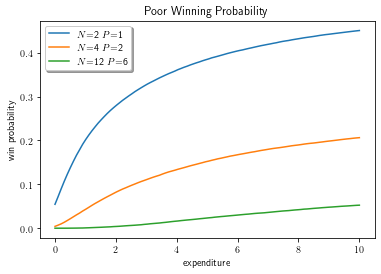
\includegraphics[width=5in]{figures/poor_winning_probability_over_n_1_to_2}
\par\end{centering}
\caption{\label{fig:Probability-to-win-for-poor-with-N}Probability to win
for poor participant with increasing number of participants}
\end{figure}

\begin{figure}
\begin{centering}
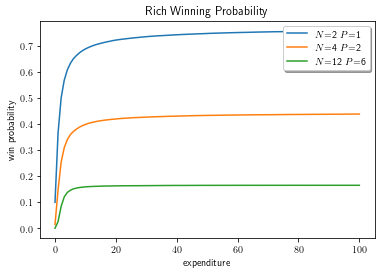
\includegraphics[width=5in]{figures/rich_winning_probability_over_n_1_to_2}
\par\end{centering}
\caption{\label{fig:Probability-to-win-for-rich-with-N}Probability to win
for rich participant  with increasing number of participants}
\end{figure}


\subsection{\label{subsec:Two-player-Discrete-Model}Equilibrium Conditions}

\noindent

The solution follows by setting total number of participants $N=2$
and the number of poor participants $P=1$ in Equations \ref{eq:CaseI_general},
\ref{eq:CaseII_general} and \ref{eq:CaseIV_general} above. As before,
a participant takes advantage of the skills with weight $1-\mu$ only
by spending an amount $\overline{\nu}$ and can decide to avoid the
expenditure altogether in order to invest it towards the savings instead.
The different probabilities in Case I, II, III and IV are discussed
before presenting the role of an additive intertemporal diminishing
utility from accumulated wealth. Recall that the behaviour of both
participants depends only on $\nu_{1},\nu_{2}$ - as they are unaware
of $r_{i},s_{i}$ before they participate. 

An important result for the closed-form solution is the probability
distribution (CDF) of $x_{i}\equiv\mu r_{i}+(1-\mu)s_{i}$ under assumption
$\mu<1-\mu$ (for independent variables $r_{i}$ and $s_{i}$ that
are uniformly distributed between 0 and 1) that is detailed in Appendix
\ref{sec:appendix_theorertical_1}.

\begin{align*}
F_{X}(x) & =P(x_{k}<x)=P(r_{k}\mu+s_{k}(1-\mu)<x)=\begin{cases}
\frac{x^{2}}{2\mu(1-\mu)} & 0<x<\mu\\
\frac{x-\mu/2}{1-\mu} & \mu<x<1-\mu\\
1-\frac{(x-1)^{2}}{2\mu(1-\mu)} & 1-\mu<x<1\\
0 & \text{otherwise}
\end{cases}
\end{align*}

Above probabilities under Case I, II, III and IV are now discussed
further.

\subsubsection*{Case I}

In Case I, the poor participant can win when her raw-talent $r_{1}$
is higher than of the total score of rich participant (who competes
with acquired skills). The poor participant is priced out of accessing
any skills $s$ in her score so that the skills $s>0$ is only true
for the rich participant having $\nu_{2}$ $=\overline{\nu}$. Thus,
the poor participant with raw-talent $r_{1}$ can win with the following
probability

\begin{align*}
P(\text{win}|r_{1}) & =P(\mu r_{2}+(1-\mu)s_{2}<\mu r_{1})=F_{X}(\mu r_{1})
\end{align*}

Notice that $\mu r_{1}<\mu<1-\mu<1$ is implied due to $\mu<\frac{1}{2}$
(and $r_{1}\in(0,1)$ ). The probability that the total score $\mu r_{2}+(1-\mu)s_{2}$
does not exceed $\mu r_{1}$ implies that only the first part of the
piece-wise function for $F_{X}(x)$ needs to be considered. Therefore,
using $P(\text{win}|r_{1})=\frac{\mu^{2}r_{1}^{2}}{2\mu(1-\mu)}$,
we evaluate $P_{1}(\text{win})$ as 
\begin{align*}
P_{1}(\text{win})=\int_{0}^{1}P(\text{win}|r_{1})dr_{1} & =\frac{\mu}{6(1-\mu)}
\end{align*}
 

%integrate (mu^2*r^2,r,0,1)/(2*mu*(1-mu)) gives \frac{\mu}{6(1-\mu)}
% for .2, the probability is .03125. The MC gives .03126 . 

Since only one of the participants can win, the probability $P_{2}(\text{win})$
for the rich participant to win is simply $1-P_{1}(\text{win})$.
The following thus applies to all other cases (i.e. Cases II, III
and IV).

\begin{align}
P_{2}(\text{win}) & =1-P_{1}(\text{win})\label{eq:two_player_rich_probability}
\end{align}


\subsubsection*{Case II}

In Case II, the rich person does not participate ($\nu_{2}=0$) and
both the poor participants have the skills-advantage in the game.
A poor participant wins by having the total score higher than the
raw-talent of the rich participant (who does not acquire skills with
investment). Representing $x_{i}\equiv\mu r_{i}+(1-\mu)s_{i}$, we
have the following probability for the poor participant to win

\begin{align*}
P(\text{win}|r_{1},s_{1}) & =P(\mu r_{2}<\mu r_{1}+(1-\mu)s_{1})
\end{align*}

Notice that $P(\mu r_{2}<\mu r_{1}+(1-\mu)s_{1})$ (i.e. $P(r_{2}<r_{1}+(\frac{1}{\mu}-1)s_{1})$
) is $1$ after $r_{1}+(\frac{1}{\mu}-1)s_{1}>1$ ( or $\mu r_{1}+(1-\mu)s_{1}>\mu)$
and $\frac{1}{\mu}$ in the interval $(0,\mu)$ (this is because $r_{2}\in(0,1)$
). In other words, 

\begin{align*}
P(r_{2}<r_{1}+(1/\mu-1)s_{1}) & =\begin{cases}
\frac{x_{1}}{\mu} & 0<x_{1}<\mu\\
1 & \text{otherwise}
\end{cases}
\end{align*}

The probability to win for the poor participant can be written as
(see Appendix \ref{sec:appendix_theorertical_1})

\begin{align*}
P(\text{win}|r_{1},s_{1}) & =\begin{cases}
\frac{x_{1}}{\mu} & 0<x<\mu\\
1 & \mu<x_{1}<1-\mu\\
1 & 1-\mu<x_{1}<1\\
0 & \text{otherwise}
\end{cases}
\end{align*}

Using double-integral properties (see Appendix \ref{sec:appendix_theorertical_2}),
the total probability to win $P_{1}(\text{win})$ for a poor participant
is evaluated as follows

\begin{multline*}
P_{1}(\text{win})=\int_{s_{1}=0}^{s_{1}=1}\int_{r_{1}=0}^{r_{1}=1}P(\text{win}|r_{1},s_{1})ds_{1}dr_{1}=\int_{r_{1}=0}^{r_{1}=1}{\int_{s_{1}=0}^{s_{1}=\frac{\mu(1-r_{1})}{1-\mu}}\ \frac{(\mu r_{1}+(1-\mu)s_{1})}{\mu}ds_{1}dr_{1}}\\
+\int_{r_{1}=0}^{r_{1}=1}{\int_{s_{1}=\frac{\mu(1-r_{1})}{1-\mu}}^{s_{1}=1-\frac{\mu r_{1}}{1-\mu}}1\ ds_{1}dr_{1}}\\
+\int_{r_{1}=0}^{r_{1}=1}{\int_{s_{1}=1-\frac{\mu r_{1}}{1-\mu}}^{s_{1}=1}1\ ds_{1}dr_{1}}\\
=\frac{\mu}{3(1-\mu)}+\frac{1-2\mu}{1-\mu}+\frac{\mu}{2(1-\mu)}\\
=\frac{2\mu}{6(1-\mu)}+\frac{6(1-2\mu)}{6(1-\mu)}+\frac{3\mu}{6(1-\mu)}=\frac{6-7\mu}{6(1-\mu)}
\end{multline*}

The probability $P_{2}(\text{win})$ for the rich participant to win
follows from Equation \ref{eq:two_player_rich_probability}.

\subsubsection*{Case III }

In Case III, when neither the rich nor the poor participate in the
game, then the game depends only on raw-talents and both participants
have the same probability $\frac{1}{2}$ to win the game. This is
because $\int_{r_{i}=0}^{r_{i}=1}P(\text{win}|r_{i})dr_{i}=\frac{r_{i}^{2}}{2}|_{0}^{1}=\frac{1}{2}$.
Both the poor and rich participant have the same total probability
$\frac{1}{2}$ to win. 

\subsubsection*{Case IV}

In Case IV, when both rich and poor participants set $\nu_{1}=\nu_{2}=\overline{\nu}$,
then the poor participant can win only if her score $x_{i}$ is above
that of the rich participant. Therefore, 

\begin{multline*}
P(\text{win}|r_{1},s_{1})=P(\mu r_{2}+(1-\mu)s_{2}<\mu r_{1}+(1-\mu)s_{1})\\
=F_{X}(x_{1})
\end{multline*}

\begin{align*}
P(\text{win}|r_{1},s_{1}) & =\begin{cases}
\frac{x_{1}^{2}}{2\mu(1-\mu)} & 0<x_{1}<\mu\\
\frac{x_{1}-\mu/2}{1-\mu} & \mu<x_{1}<1-\mu\\
1-\frac{(x_{1}-1)^{2}}{2\mu(1-\mu)} & 1-\mu<x_{1}<1\\
0 & \text{otherwise}
\end{cases}
\end{align*}

While this integral can be evaluated based on symmetry arguments (
since $x_{i}$ is also randomly distributed), the integral $\int_{s_{1}=0}^{s_{1}=1}\int_{r_{1}=0}^{r_{1}=1}P(\text{win}|r_{1},s_{1})dr_{1}ds_{1}$
also evaluates to $\frac{1}{2}$ (see Appendix \ref{sec:appendix_theorertical_2})

\begin{multline*}
\int_{s=0}^{s=1}\int_{r=0}^{r=1}F_{X}(x_{1})ds_{1}dr_{1}=\int_{r_{1}=0}^{r_{1}=1}{\int_{s_{1}=0}^{s_{1}=\frac{\mu(1-r)}{1-\mu}}\frac{(\mu r_{1}+(1-\mu)s_{1})^{2}}{2\mu(1-\mu)}\ ds_{1}dr_{1}}\\
+\int_{r_{1}=0}^{r_{1}=1}{\int_{s_{1}=\frac{\mu(1-r)}{1-\mu}}^{s_{1}=1-\frac{\mu r}{1-\mu}}(\frac{\mu r_{1}+(1-\mu)s_{1}-\mu/2}{1-\mu})\ ds_{1}dr_{1}}\\
+\int_{r_{1}=0}^{r_{1}=1}{\int_{s_{1}=1-\frac{\mu r}{1-\mu}}^{s_{1}=1}(1-\frac{(\mu r_{1}+(1-\mu)s_{1}-1)^{2}}{2\mu(1-\mu)})\ ds_{1}dr_{1}}\\
=\frac{\mu^{2}}{8(1-\mu)^{2}}+\frac{1-2\mu}{2(1-\mu)}+\frac{(4-5\mu)\mu}{8(1-\mu)^{2}}=\frac{4(1-\mu)^{2}}{8(1-\mu)^{2}}=\frac{1}{2}
\end{multline*}

% For part A,  integrate( integrate((mu *r + (1-mu)*s)^2/(2*mu*(1-mu)),s,0,mu*(1-r)/(1-mu)) , r, 0,1) gives \frac{\mu^2}{8(1-\mu)^2}
% For part B, integrate (integrate( ((mu * r + (1-mu) *s - mu /2 )/(1-mu) ),s,mu*(1-r)/(1-mu),1-mu*r/( 1-mu)) , r, 0, 1)  gives \frac{1-2\mu}{2(1-\mu)}
% For part C, integrate(integrate( (1- ((mu *r  + (1-mu) * s)-1)^2/(2*mu*(1-mu))), s, 1-mu *r /(1-mu),1),r,0,1) gives \frac{(4-5\mu)\mu}{8(1-\mu)^{2}}
% simplified with  x^2 +(1-2*x)*(1-x)*4+(4-5*x)*x which gives 4(1-x)^2

\begin{figure}
\begin{centering}
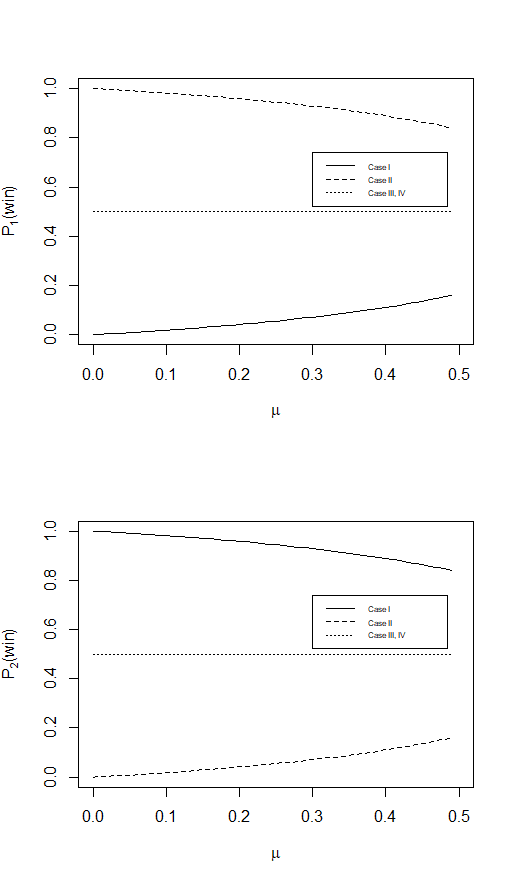
\includegraphics[width=4in]{figures/winprob_with_mu_1_to_2}
\par\end{centering}
\caption{\label{fig:Probability-of-winning}Probability of winning $P_{1}(\text{win})$,
$P_{2}(\text{win})$ for poor and rich participants with varying $\mu$}
\end{figure}

As is clear from Figure \ref{fig:Probability-of-winning} and above
results (see summaries in Tables \ref{tab:Results_summary_poor} and
\ref{tab:Results_summary_rich}), the condition $\mu<1/2$ - indicating
that curated skills are given more importance that raw-talent in the
competitions - means that the poor participant is strictly better
off (than facing probability $1/2$) if she participates while the
rich participant doesn't participate (Case II). Also, the poor participant
is better off participating for $\mu<\frac{1}{2}$ when the rich participant
does participate as it raises the probability to $1/2$. That the
competition becomes uncompetitive both when threshold $\overline{\nu}$
falls too much (letting both participants participate) or rises too
much (letting both participants withdraw) also follows from the properties
of the winning probability.

Notice that the rich participant could withdraw and face either $1/2$
or lower probability (when the poor participant participates). By
participating, therefore, the rich participant would either face probability
$1/2$ (when poor participant also participates) or better (if the
poor participant withdraws). Considering the probabilities alone,
the rich participant would always participate. If the rich participant
always participates, then so long as budget constraints permit, the
poor participant is also better off participating since not participating
brings her probability to win below $1/2$. If the utility was from
probability alone, then both participants would participate and face
$1/2$ probability.

However, it's not the probability to win that the participants optimise
(maximise). A more accurate representation of the real-world is a
game where participants face a finite life-time and utility from accumulated
assets instead. Thus, what follows is the case where the participants
optimise an intertemporally additive utility over their life-time.
The life-time in the model is represented with two time-horizons -
where the second-time horizon is one before the end of life when all
wealth accumulated by either participant must disappear. With no accumulations
at the end of life, both rich and poor participants must decide to
spend all their incomes $y_{1}$ or $y_{2}$ (for poor and rich participants
respectively so that $y_{1}<y_{2}$) towards the promotion game. In
the first-stage, however, the participants decide the amount to be
spent towards promotion based upon the utility from wealth they obtain
across the two time-horizons that span their lifetime. For the poor
participant, the total utility to be optimised (assuming EUT) under
the intertemporally additive utility $u(\cdot)$, a winning probability
function $W(x)$ (for expenditure $x$) and a discount-factor $\delta$
is 

\begin{align*}
u(y_{1}-\nu_{1})+\frac{1}{\delta}((1-W(y_{1}))u(y_{1})+W(y_{1})u(y_{2}))
\end{align*}

Similarly, for the rich participant, the total utility to be optimised
(assuming EUT) is 
\begin{align*}
u(y_{2}-\nu_{2})+\frac{1}{\delta}((1-W(y_{2}))u(y_{1})+W(y_{2})u(y_{2}))
\end{align*}

\begin{table}[H]
\begin{centering}
\begin{tabular}{>{\centering}p{0.7in}>{\centering}p{0.7in}>{\raggedright}m{1.5in}|>{\raggedright}m{1.5in}}
 &  & \multicolumn{1}{>{\raggedright}m{1.5in}}{Poor} & participant\tabularnewline
\begin{singlespace}
\end{singlespace}
 & \begin{singlespace}
\end{singlespace}
 & \begin{singlespace}
\textit{\small{}withdraws}
\end{singlespace}
 & \begin{singlespace}
\textit{\small{}participates}
\end{singlespace}
\tabularnewline
\begin{singlespace}
Rich
\end{singlespace}
 & \begin{singlespace}
\textit{\small{}withdraws}
\end{singlespace}
 & \multirow{1}{1.5in}{Case III} & Case II\tabularnewline
\cline{3-4} \cline{4-4} 
\begin{singlespace}
Participant
\end{singlespace}
 & \begin{singlespace}
\textit{\small{}participates}
\end{singlespace}
 & \begin{singlespace}
Case I
\end{singlespace}
 & \begin{singlespace}
Case IV
\end{singlespace}
\tabularnewline
\end{tabular}
\par\end{centering}
\caption{\label{tab:prisoners_dilemma_cases}Cases I,II, III, IV as participant
strategies}
\end{table}

\begin{table}[H]
\begin{raggedright}
{\footnotesize{}}%
\begin{tabular*}{1.2in}{@{\extracolsep{\fill}}>{\raggedright}p{0.5in}>{\raggedright}p{0.4in}>{\centering}m{2.5in}|>{\raggedright}m{2.2in}}
 &  & \multicolumn{1}{>{\centering}m{2.5in}}{\begin{onehalfspace}
{\footnotesize{}Poor}
\end{onehalfspace}
} & \begin{onehalfspace}
{\footnotesize{}participant}
\end{onehalfspace}
\tabularnewline
 &  & \begin{onehalfspace}
\textit{\footnotesize{}withdraws}
\end{onehalfspace}
 & \begin{onehalfspace}
\textit{\footnotesize{}participates}
\end{onehalfspace}
\tabularnewline
{\footnotesize{}Rich}\\
{\footnotesize{}participant} & \textit{\footnotesize{}withdraws} & {\footnotesize{}
\begin{gather*}
u(y_{2})+\frac{(1-\frac{P}{N})u(y_{2})+\frac{P}{N}u(y_{1})}{\delta}
\end{gather*}
}\\
{\footnotesize{}
\begin{gather*}
u(y_{1})+\frac{(1-\frac{P}{N})u(y_{2})+\frac{P}{N}u(y_{1})}{\delta}
\end{gather*}
} & {\footnotesize{}
\begin{gather*}
u(y_{2})+\frac{u(y_{2})p_{2}'+(1-p_{2}')u(y_{1})}{\delta}
\end{gather*}
}\\
{\footnotesize{}
\begin{gather*}
u(y_{1}-\overline{\nu})+\frac{u(y_{2})p_{1}'+(1-p_{1}')u(y_{1})}{\delta}
\end{gather*}
}\tabularnewline
\cline{2-4} \cline{3-4} \cline{4-4} 
 & \textit{\footnotesize{}participates} & {\footnotesize{}
\begin{gather*}
u(y_{2}-\overline{\nu})+\frac{p_{2}u(y_{2})+(1-p_{2})u(y_{1})}{\delta}
\end{gather*}
}\\
{\footnotesize{}
\begin{gather*}
u(y_{1})+\frac{p_{1}u(y_{2})+(1-p_{1})u(y_{1})}{\delta}
\end{gather*}
} & {\footnotesize{}
\begin{gather*}
u(y_{2}-\overline{\nu})+\frac{(1-\frac{P}{N})u(y_{2})+\frac{P}{N}u(y_{1})}{\delta}
\end{gather*}
 }\\
{\footnotesize{}
\begin{gather*}
u(y_{1}-\overline{\nu})+\frac{(1-\frac{P}{N})u(y_{2})+\frac{P}{N}u(y_{1})}{\delta}
\end{gather*}
}\tabularnewline
\end{tabular*}{\footnotesize{}fol}{\footnotesize\par}
\par\end{raggedright}
\caption{\label{tab:prisoners_dilemma}Utility from two periods for (rich,poor)
participants - at the start of the first-period (with $P$ poor participants
among $N$ total participants)}
\end{table}

\noindent

With above utilities, the conditions for whether the Case I, II, III,
IV can become Nash equilibria (see Table \ref{tab:prisoners_dilemma_cases})
are now discussed. A discussion of the implications for the effect
of income differences on expenditure towards status then follows.
It is worth remarking that the discussion of the effect of the threshold
$\overline{\nu}$ and the income differences $y_{2}-y_{1}$ on participation
(expenditure) assumes that the exogenous parameter $\mu$ is stable
with respect to short-term changes in threshold investment $\overline{\nu}$
as well as disposable incomes $y_{1},y_{2}$. 

For ease of notation we define $p_{1},p_{2},p_{1}'$ and $p_{2}'$
- which correspond to the\textbf{ two-player }model discussed above.

\begin{gather}
p_{1}\equiv\frac{\mu}{6(1-\mu)}\nonumber \\
p_{2}\equiv1-p_{1}\nonumber \\
p_{1}'\equiv\frac{6-7\mu}{6(1-\mu)}\label{eq:probabilities_2player}\\
p_{2}'\equiv1-p_{1}'\nonumber 
\end{gather}
 

The choices for the poor and rich participants using a general intertemporally
additive function $u(A)$ (for assets $A$) are shown in Table \ref{tab:prisoners_dilemma}.
As we can verify from Figure \ref{fig:Probability-of-winning} that
we have $p_{1}<1/2<p_{2}$ and $p_{1}'>1/2>p_{2}'$ for all values
of $\mu<1/2$.

\begin{gather}
\text{Given }\mu<1/2,\text{we have}\label{eq:probability_inequality}\\
p_{1}<1/2<p_{2}\nonumber \\
p_{1}'>1/2>p_{2}'\nonumber 
\end{gather}
 

Notice the Table \ref{tab:prisoners_dilemma} represents the condition
when the budget is non-binding i.e. the poor participant is able to
spend $\overline{\nu}$. i.e. $\overline{\nu}<y_{1}<y_{2}$. When
the poor participant faces a binding constraint i.e. $y_{1}<\overline{\nu}<y_{2}$
, then the rich participant knows that the best case probability to
win for the poor participant is $\frac{1}{2}$. The rich participant's
decision to participate would depend only on utility from savings
and the relative advantage from gain in probability. This is elaborated
further in Section \ref{subsec:Binding-constraint}.

Since the number of poor participants is likely to be higher than
that of rich participants in a typical competition, the unequal number
of poor and rich participants seems also worth considering in the
model. Setting $N=3,P=2$ in the equations \ref{eq:CaseI_general},
\ref{eq:CaseII_general} and \ref{eq:CaseIV_general}, for example,
one can interpret the \textbf{three-player} model with the following
values of $p_{1},p_{2},p_{1}'$ and $p_{2}'$ 

\begin{gather}
p_{1}=\frac{\mu}{8(1-\mu)}\nonumber \\
p_{2}=1-2p_{1}\nonumber \\
p_{1}'=\frac{19\mu^{2}-40\mu+20}{40(1-\mu)^{2}}\label{eq:probabilities_3player}\\
p_{2}'=1-2p_{1}'\nonumber 
\end{gather}

\begin{table}[H]
\begin{centering}
\begin{tabular}{|>{\centering}p{1cm}|>{\centering}p{3cm}|>{\centering}p{4cm}|>{\raggedright}p{7cm}|}
\hline 
Case & Description & Probability of poor participant to win & Response to $\mu$\tabularnewline
\hline 
\hline 
\begin{onehalfspace}
I
\end{onehalfspace}
 & \begin{onehalfspace}
Only rich invest in skills
\end{onehalfspace}
 & 
\begin{gather*}
\frac{\mu}{6(1-\mu)}
\end{gather*}
 & \begin{onehalfspace}
With higher $\mu$, the participants with raw-talent get rewarded.
The probability to win increases with higher $\mu$ for the poorer
participant.
\end{onehalfspace}
\tabularnewline
\hline 
\begin{onehalfspace}
II
\end{onehalfspace}
 & \begin{onehalfspace}
Only poor invest in skills
\end{onehalfspace}
 & 
\begin{gather*}
\frac{6-7\mu}{6(1-\mu)}
\end{gather*}
 & \begin{onehalfspace}
With higher $\mu$, the poor participants with access to skills get
rewarded. Therefore, The probability to win decreases with higher
$\mu$ for the poorer participant.
\end{onehalfspace}
\tabularnewline
\hline 
\begin{onehalfspace}
III,IV
\end{onehalfspace}
 & \begin{onehalfspace}
Neither or Both invest in skills
\end{onehalfspace}
 & 
\begin{gather*}
\frac{1}{2}
\end{gather*}
 & \begin{onehalfspace}
Probabilty to win is independent of $\mu$.
\end{onehalfspace}
\tabularnewline
\hline 
\end{tabular}
\par\end{centering}
\caption{\label{tab:Results_summary_poor}The probability of winning for the
poor participant in the 3-player model}
\end{table}

% Poor participant
% require(latex2exp)
% x = seq(0,.499,.01); plot(0,0,type='l',xlim=c(0,.5),ylim=c(0,1),xlab=TeX("$\\mu$"),ylab=TeX("P(win)")); 
% lines(x,(x*(x^2-2*x-3)+4)/(12*(1-x)),type='l',lty=1) # only rich
% lines(x,(-16*x**3 + 65*x**2 - 90*x + 40 )/( 120 * (1-x)**2),lty=2) # only poor
% lines(x,rep(1/3,length(x)),lty=3) # neither or both
% legend(0.3, .7,legend=TeX(paste("Case",c("I","II","III,IV"))),lty=c(1,2,3),cex=.7) 

\begin{table}[H]
\begin{centering}
\begin{tabular}{|>{\centering}p{1cm}|>{\centering}p{3cm}|>{\raggedright}m{4cm}|>{\raggedright}p{7cm}|}
\hline 
Case & Description & Probability of rich participant to win & Response to $\mu$\tabularnewline
\hline 
\hline 
\begin{onehalfspace}
I
\end{onehalfspace}
 & \multirow{1}{3cm}{\begin{onehalfspace}
Only rich \\
invest in skills
\end{onehalfspace}
} & \multirow{1}{4cm}{\begin{onehalfspace}
\begin{gather*}
1-\frac{\mu}{6(1-\mu)}
\end{gather*}
\end{onehalfspace}
} & \begin{onehalfspace}
With higher $\mu$, the participants with raw-talent get rewarded.
Therefore, the probability to win decreases with higher $\mu$ for
the rich participant.
\end{onehalfspace}
\tabularnewline
\hline 
\begin{onehalfspace}
II
\end{onehalfspace}
 & \begin{onehalfspace}
Only poor invest in skills
\end{onehalfspace}
 & \begin{onehalfspace}
\begin{gather*}
1-\frac{6-7\mu}{6(1-\mu)}
\end{gather*}
\end{onehalfspace}
 & \begin{onehalfspace}
With higher $\mu$, the poor participants with access to skills get
rewarded. Therefore, the probability to win increases with higher
$\mu$ for the rich participant.
\end{onehalfspace}
\tabularnewline
\hline 
\begin{onehalfspace}
III,IV
\end{onehalfspace}
 & \begin{onehalfspace}
Neither or Both invest in skills
\end{onehalfspace}
 & \begin{onehalfspace}
\begin{gather*}
\frac{1}{2}
\end{gather*}
\end{onehalfspace}
 & \begin{onehalfspace}
Probabilty to win is independent of $\mu$.
\end{onehalfspace}
\tabularnewline
\hline 
\end{tabular}
\par\end{centering}
\caption{\label{tab:Results_summary_rich}The probability of winning for the
rich participant in the 3-player model}
\end{table}

% Rich participant
% require(latex2exp)
% x = seq(0,.499,.01); plot(0,0,type='l',xlim=c(0,.5),ylim=c(0,1),xlab=TeX("$\\mu$"),ylab=TeX("P(win)")); 
% lines(x,1-(x*(x^2-2*x-3)+4)/(6*(1-x)),type='l',lty=1) # only rich
% lines(x,1-(-16*x**3 + 65*x**2 - 90*x + 40 )/( 60 * (1-x)**2),lty=2) # only poor
% lines(x,rep(1/3,length(x)),lty=3) # neither or both
% legend(0.3, .7,legend=TeX(paste("Case",c("I","II","III,IV"))),lty=c(1,2,3),cex=.7) 

Comparing these probabilities with those from the 2-player model in
Equation \ref{eq:probabilities_2player} (also listed in Tables \ref{tab:Results_summary_poor}
and \ref{tab:Results_summary_rich}), it can be seen that the probability
to win for the poor participant in the 3-player model is lower with
respect to the Case III probability (i.e. $1/N$). Likewise, the probability
for the rich participant to win is higher in the 3-player model with
respect to the Case III probability ($1/N$). The implications for
the unequal number of poor and rich participants are further discussed
in Section \ref{subsec:Non-Binding-constraint}.

\begin{figure}
\begin{centering}
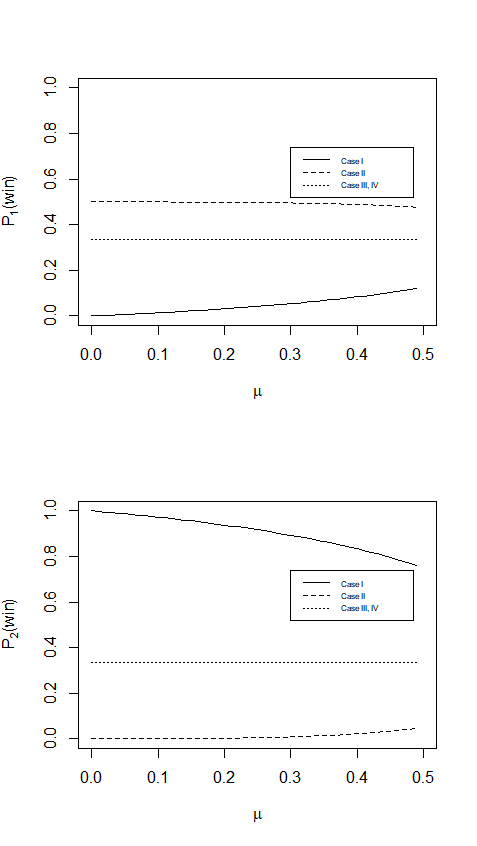
\includegraphics[width=4in]{figures/winprob_with_mu_2_to_3}
\par\end{centering}
\caption{\label{fig:Probability-of-winning-2-to-3}Probability of winning $P_{1}(\text{win})$,
$P_{2}(\text{win})$ for poor and rich participants with varying $\mu$}
\end{figure}


\subsubsection{\label{subsec:Binding-constraint}Binding constraint}

\noindent

Assuming EUT participants, consider the simpler case of binding constraint
$y_{1}<\overline{\nu}<y_{2}$ first . With the assumption of a stability
in long-term participant behaviour (which itself is a result of observed
probability of success), mixed-strategies are not considered relevant
in the current set up. Considering pure strategies for participation,
the rich participant would thus participate only when the utility
from participating would be higher than from not participating i.e.
$u(y_{2}-\overline{\nu})+\frac{p_{2}u(y_{2})+(1-p_{2})u(y_{1})}{\delta}>u(y_{2})+\frac{u(y_{2})+u(y_{1})}{2\delta}$
. This results in the following condition

\begin{align*}
\frac{(p_{2}-1/2)(u(y_{2})-u(y_{1}))}{\delta} & >u(y_{2})-u(y_{2}-\overline{\nu})
\end{align*}

With income differences being the same an increase in participation
cost $\overline{\nu}$ discourages participation since RHS increases
with $\overline{\nu}$ ($\because u(y_{2}-\overline{\nu})$ is decreasing
in $\overline{\nu}$) and may fail the above condition. Similarly,
with participation cost $\overline{\nu}$ being the same, an increase
in income-difference $y_{2}-y_{1}$ is in the rich participant's interest
whereas a narrowing of income differences reduces incentive for the
participant to participate by possibly failing the above condition.
All else being the same, higher impatience (lower time-discounted
value of money or a higher $\delta$) would also discourage participation.
Therefore, when budget is binding for the poor participant i.e. if
the poor participant cannot participate due to $y_{1}<\overline{\nu}$,
then narrower income differences, higher participation costs and higher
patience for savings (common for both rich and poor participants)
all encourage the rich participant to withdraw from the game. This
also means that wider income differences ($y_{2}-y_{1}$) combined
with lower participation costs ($\overline{\nu}$) may together help
maintain the equilibrium where only the rich participates. Similarly,
wider income differences ( higher $y_{2}-y_{1}$ ) and more patience
for savings (higher $\delta$) would together maintain the incentive
for the rich participant to participate. These conclusions very much
fit with the sociological observations made in the literature about
status \cite{HirschSocialLimits,GalbraithEssential}.

\subsubsection{\label{subsec:Non-Binding-constraint}Non-Binding constraint}

\noindent

When budget is non-binding, then participation of the rich participant
is her dominant strategy if the condition is also $u(y_{2})+\frac{u(y_{2})p_{2}'+(1-p_{2}')u(y_{1})}{\delta}<u(y_{2}-\overline{\nu})+\frac{u(y_{2})+u(y_{1})}{2\delta})$
i.e. 

\begin{align*}
\frac{(1/2-p_{2}')(u(y_{2})-u(y_{1}))}{\delta} & >u(y_{2})-u(y_{2}-\overline{\nu})
\end{align*}

The inferences on how $y_{2}-y_{1}$, $\overline{\nu}$ and $\delta$
influence the participation (see Section \ref{subsec:Binding-constraint})
remain the same for the above condition. To discuss the more general
Nash equilibria, consider the conditions for all of the Cases I, II,
III and IV to become a Nash equilibrium. For ease of notation we define
the following for a given $\overline{\nu},y_{1}$ and $y_{2}$

\begin{align*}
U_{1} & \equiv u(y_{1})-u(y_{1}-\overline{\nu})
\end{align*}

\begin{align*}
U_{2} & \equiv u(y_{2})-u(y_{2}-\overline{\nu})
\end{align*}

One could view $U_{1}$ and $U_{2}$ as the immediate gain in wealth
utility from withdrawing. If $u(\cdot)$ represents a diminishing
utility, then it is also necessary for $y_{1}<y_{2}$ that 

\begin{align*}
U_{2} & <U_{1}
\end{align*}

Consider now that conditions for Case I to be a Nash Equilibrium.
If Case I were to be a Nash equilibrium, then for the rich participant's
decision to participate, the poor participant must get more utility
from withdrawing than from participating and for poor participant's
decision to withdraw, the rich must get more utility from participating
than from withdrawing. The following conditions \footnote{$u(y_{1})+\frac{p_{1}u(y_{2})+(1-p_{1})u(y_{1})}{\delta}>u(y_{1}-\overline{\nu})+\frac{\frac{1}{N}u(y_{2})+\frac{1}{N}u(y_{1})}{\delta}\Rightarrow u(y_{1})-u(y_{1}-\overline{\nu})>\frac{(\frac{1}{N}-p_{1})(u(y_{2})-u(y_{1}))}{\delta}$
and $u(y_{2}-\overline{\nu})+\frac{p_{2}u(y_{2})+(1-p_{2})u(y_{1})}{\delta}>u(y_{2})+\frac{\frac{1}{N}u(y_{2})+\frac{1}{N}u(y_{1})}{\delta}\Rightarrow u(y_{2})-u(y_{2}-\overline{\nu})<\frac{(p_{2}-1/N)(u(y_{2})-u(y_{1}))}{\delta}$} must therefore hold simultaneously

\begin{gather}
\frac{(\frac{1}{N}-p_{1})(u(y_{2})-u(y_{1}))}{\delta}<U_{1}\nonumber \\
U_{2}<\frac{(p_{2}-1/N)(u(y_{2})-u(y_{1}))}{\delta}\label{eq:caseI_inequalities}
\end{gather}

% (\frac{(\frac{1}{3}-p_{1})(u(y_{2})-u(y_{1}))}{\delta},\frac{(p_{2}-1/3)(u(y_{2})-u(y_{1}))}{\delta})

Since $p_{2}-\frac{1}{N}\ge\frac{1}{N}-p_{1}$ (strict inequality
follows when the number of poor participants $P$ is higher than that
for rich participants $N-P$ e.g., with $N=3$ and $P=2$), this is
a fairly general condition for the equilibrium. An increase in $U_{1}$
due to higher $\overline{\nu}$ does not change the equilibrium conditions
so long as the corresponding rise $U_{2}$ (due to higher $\overline{\nu}$
) does not affect the second inequality. In other words, a higher
$\overline{\nu}$ favours the equilibrium (Case I) so long as there
is an incentive for the rich to participate. Likewise, a decrease
in $\overline{\nu}$ would be favourable for the equilibrium (Case
I) so long as the poor participants do not also have an incentive
to participate. 

Similar effects can be seen with income differences $y_{2}-y_{1}$
(which increase $u(y_{2})-u(y_{1})$ as well as $\frac{U_{2}}{U_{1}}$)
if we rewrite Equation \ref{eq:caseI_inequalities} as 

\begin{gather*}
\frac{(\frac{1}{N}-p_{1})}{\delta}<\frac{U_{1}}{u(y_{2})-u(y_{1})}\\
\frac{U_{2}}{(u(y_{2})-u(y_{1}))}<\frac{(p_{2}-1/N)}{\delta}
\end{gather*}

Limiting our attention to cases when $\overline{\nu}<y_{1}$, higher
$y_{2}$ for fixed $y_{1}$ decreases $\frac{U_{2}}{u(y_{2})-u(y_{1})}$and
makes it more likely for the rich to participate while it also decreases$\frac{U_{1}}{u(y_{2})-u(y_{1})}$
by raising the stakes enough for the poor to participate (making it
less likely for first inequality to be fulfilled). It is easy to see
that higher impatience $\delta$ encourages both poor and rich to
withdraw. As would be evident, the equilibrium conditions corresponding
to Case II are far more stringent.

If Case II is a Nash Equilibrium, then for rich's decision to withdraw,
the poor participant should get more utility from participating than
from withdrawing and for poor participant's decision to participate,
the rich participant should get more utility from withdrawing than
from participating. This means that the following hold \footnote{$u(y_{1}-\overline{\nu})+\frac{p_{1}'u(y_{2})+(1-p_{1}')u(y_{1})}{\delta}>u(y_{1})+\frac{\frac{1}{N}u(y_{2})+\frac{1}{N}u(y_{1})}{\delta}\Rightarrow u(y_{1})-u(y_{1}-\overline{\nu})<\frac{(p_{1}'-1/N)(u(y_{2})-u(y_{1}))}{\delta}$
and $u(y_{2})+\frac{p_{2}'u(y_{2})+(1-p_{2}')u(y_{1})}{\delta}>u(y_{2}-\overline{\nu})+\frac{\frac{1}{N}u(y_{2})+\frac{1}{N}u(y_{1})}{\delta}\Rightarrow u(y_{2})-u(y_{2}-\overline{\nu})>\frac{(1/N-p_{2}')(u(y_{2})-u(y_{1}))}{\delta}$} simultaneously, 

\begin{gather*}
U_{1}<\frac{(p_{1}'-1/N)(u(y_{2})-u(y_{1}))}{\delta}\\
U_{2}>\frac{(1/N-p_{2}')(u(y_{2})-u(y_{1}))}{\delta}
\end{gather*}

Since $\frac{(p_{1}'-1/N)(u(y_{2})-u(y_{1}))}{\delta}<\frac{(1/N-p_{2}')(u(y_{2})-u(y_{1}))}{\delta}$
, the above cannot be satisfied so long as we have a diminishing utility
which necessitates $U_{2}<U_{1}$. Thus an equilibrium with Case II
which incentivises the poor to participate but not the rich is possible
only with a reference dependent utility with $U_{1}<U_{2}$. With
$U_{1}<U_{2}$, we can write above as 

\begin{gather*}
\frac{U_{1}}{u(y_{2})-u(y_{1})}<\frac{(p_{1}'-1/N)}{\delta}<\frac{(1/N-p_{2}')}{\delta}<\frac{U_{2}}{u(y_{2})-u(y_{1})}
\end{gather*}

Notice that despite a reference-dependent utility, a higher $\overline{\nu}$
or more impatience ($\delta$) may disincentivise the poor from participation
just the same (leading to Case III). Similarly, higher income differences
(an increase in $y_{2}$ for fixed $y_{1}$) could encourage the rich
to participate by decreasing $\frac{U_{2}}{u(y_{2})-u(y_{1})}$ (leading
to Case IV). Even with the reference dependent utility, the equilibrium
with Case II remains a fragile one.

If Case III were to be a Nash-Equilibrium, then for rich participant's
decision to withdraw, poor should get more utility from withdrawing
than from participating and for poor participant's decision to withdraw,
the rich participant should get more from withdrawing than from participating.
The following should thus hold\footnote{$u(y_{1})+\frac{\frac{1}{N}u(y_{2})+\frac{1}{N}u(y_{1})}{\delta}>u(y_{1}-\overline{\nu})+\frac{p_{1}'u(y_{2})+(1-p_{1}')u(y_{1})}{\delta}\Rightarrow u(y_{1})-u(y_{1}-\overline{\nu})>\frac{(p_{1}'-\frac{1}{N})(u(y_{2})-u(y_{1}))}{\delta}$
and $u(y_{2})+\frac{\frac{1}{N}u(y_{2})+\frac{1}{N}u(y_{1})}{\delta}>u(y_{2}-\overline{\nu})+\frac{p_{2}u(y_{2})+(1-p_{2})u(y_{1})}{\delta}\Rightarrow u(y_{2})-u(y_{2}-\overline{\nu})>\frac{(p_{2}-\frac{1}{N})(u(y_{2})-u(y_{1}))}{\delta}$},

\begin{gather*}
U_{1}>\frac{(p_{1}'-\frac{1}{N})(u(y_{2})-u(y_{1}))}{\delta}\\
U_{2}>\frac{(p_{2}-\frac{1}{N})(u(y_{2})-u(y_{1}))}{\delta}
\end{gather*}

Since $p_{1}'-\frac{1}{N}\le p_{2}-\frac{1}{N}$ (strict inequality
when number of poor participants is higher), we have $\frac{(p_{1}'-\frac{1}{N})(u(y_{2})-u(y_{1}))}{\delta}<\frac{(p_{2}-\frac{1}{N})(u(y_{2})-u(y_{1}))}{\delta}$
and $U_{2}<U_{1}$ . A higher $\overline{\nu}$ pushes both $U_{2}$
and $U_{1}$ further away from participation but a fall in $\overline{\nu}$,
incentivises the rich participant to participate (leading to Case
I). 

\begin{gather*}
\frac{U_{1}}{u(y_{2})-u(y_{1})}>\frac{(p_{1}'-\frac{1}{N})}{\delta}\\
\frac{U_{2}}{u(y_{2})-u(y_{1})}>\frac{(p_{2}-\frac{1}{N})}{\delta}
\end{gather*}

Higher income differences i.e. higher $y_{2}$ for fixed $y_{1}$
also decrease $\frac{U_{2}}{u(y_{2})-u(y_{1})}$ and incentivise the
rich participant to participate (leading to an equilibrium with Case
I). Conversely, if the game is not lucrative for the rich it would
automatically be infeasible for the poor i.e. if rich withdraws then
poor automatically withdraws. If there is any net utility from playing
the game, however, Case IV is the likely equilibrium.

If Case IV were to be a Nash Equilibrium, then for rich's decision
to participate, the poor participant should get more from participating
than from withdrawing and for poor's decision to participate, the
rich participant should get more from participating than from withdrawing.
Therefore, the following\footnote{$u(y_{1}-\overline{\nu})+\frac{\frac{1}{N}u(y_{2})+\frac{1}{N}u(y_{1})}{\delta}>u(y_{1})+\frac{p_{1}u(y_{2})+(1-p_{1})u(y_{1})}{\delta}\Rightarrow u(y_{1})-u(y_{1}-\overline{\nu})<\frac{(\frac{1}{N}-p_{1})(u(y_{2})-u(y_{1}))}{\delta}$
and $u(y_{2}-\overline{\nu})+\frac{\frac{1}{N}u(y_{2})+\frac{1}{N}u(y_{1})}{\delta}>u(y_{2})+\frac{p_{2}'u(y_{2})+(1-p_{2}')u(y_{1})}{\delta}\Rightarrow u(y_{2})-u(y_{2}-\overline{\nu})<\frac{(\frac{1}{N}-p_{2}')(u(y_{2})-u(y_{1}))}{\delta}$} must hold

\begin{gather*}
U_{1}<\frac{(\frac{1}{N}-p_{1})(u(y_{2})-u(y_{1}))}{\delta}\\
U_{2}<\frac{(\frac{1}{N}-p_{2}')(u(y_{2})-u(y_{1}))}{\delta}
\end{gather*}

With $\frac{(\frac{1}{N}-p_{2}')(u(y_{2})-u(y_{1}))}{\delta}<\frac{(\frac{1}{N}-p_{1})(u(y_{2})-u(y_{1}))}{\delta}$
and $U_{2}<U_{1}$ , this equilibrium rests upon the incentive for
the poor participant to participate. So long as the poorer participant
finds the competition worthwhile, the rich would also participate. 

The above results outline how participation costs influence the investments
towards status. For very low $\overline{\nu}$, rich and poor would
both participate and for very high $\overline{\nu}$, both would withdraw.
For everything in between, the only equilibrium with a diminishing
utility from wealth is one where rich participate whereas poor don't.

The above framework also allows us to discuss the implications of
inequality for the same total wealth in the economy. As such, a segregation
where the poor never participate in the status economy seems less
favourable than one where both rich and poor participate in the status
competitions. The current chapter explains that the likely outcome
of a failure to maintain universal participation in status games (under
diminishing utility from wealth) is that of a segregation where only
the rich participate in skills leading to economic success. While
a reference-based utility (which may be encouraged with segregation)
does seem to permit an equilibrium where only the poor are concerned
with status games (with respect to skills-enhancement), the result
only suggests that a segregation of status games along with that of
incomes is another possible long-term outcome of limited participation.

\section{\label{sec:Conclusion}Conclusion}

\noindent 

The paper considers a model where status amounts to a position maintained
by the participant's social capital investments. With a decision theory
framework for uncertainty, the goal of the model has been to investigate
role of income difference on expenditures that carry some status while
also having some effect on the income mobility of the participants.
The endogenisation of status in this manner allows an understanding
of the role of income difference in status consumption in a generic
framework across cultural settings.

The foremost result from the model is that under diminishing utility
from wealth, the only two stable equilibria are those where both rich
and poor participate in status competitions and those where only rich
stand to benefit from status competitions. This delineates the limits
to the benefits to poor offered by participation in status competitions
- providing a quantitative basis for limits to social growth in literature
\cite{HirschSocialLimits,GalbraithBeyondContentment1994,GalbraithAffluent}. 

The model also allows us to understand how a withdrawal from expenditure
such as education (particularly in certain developing economies with
significantly high income differences) could be the result of a combined
effect of both participation costs and income-differences. More specifically,
high participation costs push the equilibrium to one where where only
rich participate in status-related competitions while high income
differences may still have the unlikely effect of incentivising the
poor participants to participate. Lowering of participation costs
in education (as a status game) despite a rise in income differences
may correspond to an escape from segregation of participation and
the feasbility of status competitions.

Lastly, the role of a reference-based utility adds an important caveat
to these results since contentment at lower levels of wealth could
support segregation of competitions at different income levels in
the economy. This seems also in line with many of the findings from
subjective contentment data on the belief in meritocracy and persisting
inequalities in the developed economies \cite{MijsMeritocracy2020}.

\bibliographystyle{apacite}
\bibliography{status_consumption} 

\begin{appendices}
\section{Convolution of Uniform Random Variables} \label{sec:appendix_theorertical_1}

The distribution of a convex combination $w=\mu r+(1-\mu)s$ of two
random variables $r,s$ - which are distributed according to densities
$f_{R}(r)$ and $f_{S}(s)$ - can be derived using the convolution
of two derived variables $x=\mu r$ and $y=(1-\mu)s$. If $r$ and
$s$ are uniformly distributed variables ranging from 0 to 1, then
$x$ ranges from 0 to $\mu$ and $y$ ranges from $0$ to $(1-\mu)$.
The CDF for $F_{X}(x)$ and $F_{Y}(y)$ are simply $F_{X}(x)=\frac{x}{\mu}$
, $F_{Y}(y)=\frac{y}{1-\mu}$ (respectively). Therefore, the densities
for $x$ and $y$ are $f_{X}(x)=\frac{1}{\mu}$ and $f_{Y}(y)=\frac{1}{1-\mu}$.
The density of $w$ is simple $f(w)=\int_{-\infty}^{\infty}f_{Y}(w-x)f_{X}(x)dx$.
Since , $f_{X}(x)$ is $1/\mu$ only between $0$ and $\mu$. We have
the following integral to evaluate for the convolution

\begin{align*}
f(w) & =\frac{1}{\mu}\int_{0}^{\mu}f_{Y}(w-x)dx
\end{align*}

Since $f_{Y}(y)$ is 1 only between 0 and $1-\mu$, we have the condition
$0<w-x<1-\mu\Rightarrow w-(1-\mu)<x<w$. Further, $x$ is distributed
only between 0 and $\mu$. As shown in Figure \ref{fig:convex_combo},
the integral would evaluate to the following\footnote{Notice that as a convex combination, $w$ is distributed only between
0 and 1.} under the assumption $\mu<\frac{1}{2}$.

\begin{align*}
f(w)=\frac{1}{\mu}\int_{0}^{\mu}f_{Y}(w-x)dx & =\begin{cases}
\frac{1}{\mu}\int_{0}^{w}\frac{1}{1-\mu}dx & 0<w<\mu\\
\frac{1}{\mu}\int_{0}^{\mu}\frac{1}{1-\mu}dx & \mu<w<1-\mu\\
\frac{1}{\mu}\int_{w-(1-\mu)}^{\mu}\frac{1}{1-\mu}dx & 1-\mu<w<1\\
0 & \text{otherwise}
\end{cases}
\end{align*}

This can be simplified as 

\begin{align*}
f(w) & =\begin{cases}
\frac{w}{\mu(1-\mu)} & 0<w<\mu\\
\frac{1}{1-\mu} & \mu<w<1-\mu\\
\frac{1-w}{\mu(1-\mu)} & 1-\mu<w<1\\
0 & \text{otherwise}
\end{cases}
\end{align*}

Figure \ref{fig:convex_combo_plot} shows this trapezoidal density
with $\mu$ set to $\frac{1}{5}$. The CDF $F_{X}(x)$ can be evaluated
by integrating the above density as $P(X<x)=\int_{-\infty}^{x}f(t)dt$. 

\begin{align*}
F_{X}(x) & =\begin{cases}
\frac{x^{2}}{2\mu(1-\mu)} & 0<x<\mu\\
\frac{\mu}{2(1-\mu)}+\frac{x-\mu}{1-\mu} & \mu<x<1-\mu\\
\frac{\mu^{2}}{2\mu(1-\mu)}+\frac{2\mu(1-2\mu)}{2\mu(1-\mu)}+\frac{\mu^{2}-x^{2}+2x-1}{2\mu(1-\mu)} & 1-\mu<x<1\\
0 & \text{otherwise}
\end{cases}
\end{align*}

Simplifying above, we have

\begin{align*}
F_{X}(x) & =\begin{cases}
\frac{x^{2}}{2\mu(1-\mu)} & 0<x<\mu\\
\frac{x-\mu/2}{1-\mu} & \mu<x<1-\mu\\
1-\frac{(x-1)^{2}}{2\mu(1-\mu)} & 1-\mu<x<1\\
0 & \text{otherwise}
\end{cases}
\end{align*}

\begin{figure}[H]
\begin{centering}
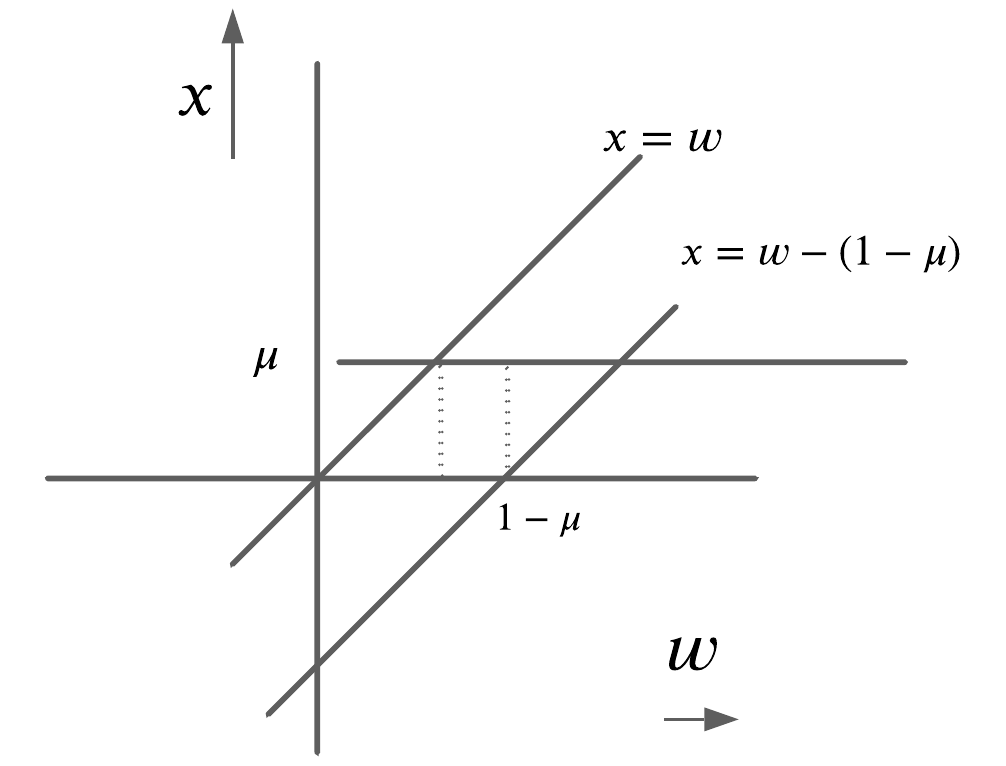
\includegraphics[width=4in]{figures/combined_density}
\par\end{centering}
\caption{\label{fig:convex_combo}Ranges of $w$ and $w-x$ for convolution
of two scaled random variables}
\end{figure}

\begin{figure}[H]
\begin{centering}
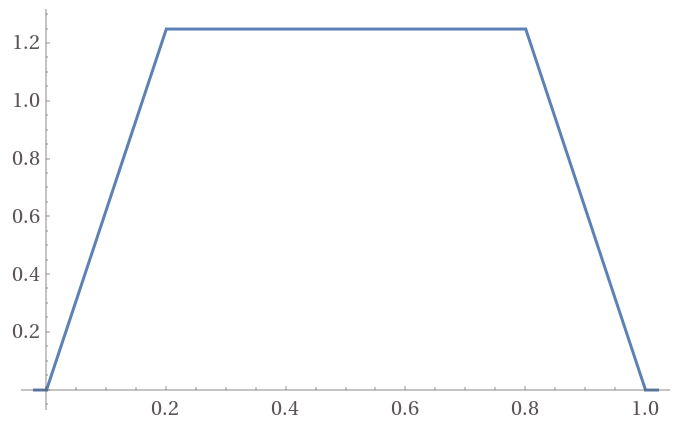
\includegraphics[width=4in]{figures/combined_density_plot}
\par\end{centering}
\caption{\label{fig:convex_combo_plot}Combined density of $w$ as the convex
combination of two random variables with $\mu=\frac{1}{5}$}
\end{figure}

\newpage
\section{$P(\text{win}|r,s)$} \label{sec:appendix_theorertical_2} 

To calculate $\int_{s=0}^{s=1}\int_{r=0}^{r=1}P(\text{win}|r,s)drds$
over the variable $x$ (where $0<r<1$ and $0<s<1$), we evaluate
the sum of three parts split by the boundaries of the piecewise function.
The three parts are shown in Figure \ref{fig:integral_boundaries}.
If $x=\mu r+(1-\mu)s$ and $F(x)$ is of the following piece-wise
form

\begin{align*}
F(x) & =\begin{cases}
A & 0<x<\mu\\
B & \mu<x<1-\mu\\
C & 1-\mu<x<1\\
0 & \text{otherwise}
\end{cases}
\end{align*}

Then the integral $\int_{s=0}^{s=1}\int_{r=0}^{r=1}F(x)drds$ can
be written as

\begin{align*}
\int_{s=0}^{s=1}\int_{r=0}^{r=1}F(x)dsdr & =\int_{r=0}^{r=1}{\int_{s=0}^{s=\frac{\mu(1-r)}{1-\mu}}A\ dsdr}+\int_{r=0}^{r=1}{\int_{s=\frac{\mu(1-r)}{1-\mu}}^{s=1-\frac{\mu r}{1-\mu}}B\ dsdr}+\int_{r=0}^{r=1}{\int_{s=1-\frac{\mu r}{1-\mu}}^{s=1}C\ dsdr}
\end{align*}

\begin{figure}[h]
\begin{centering}
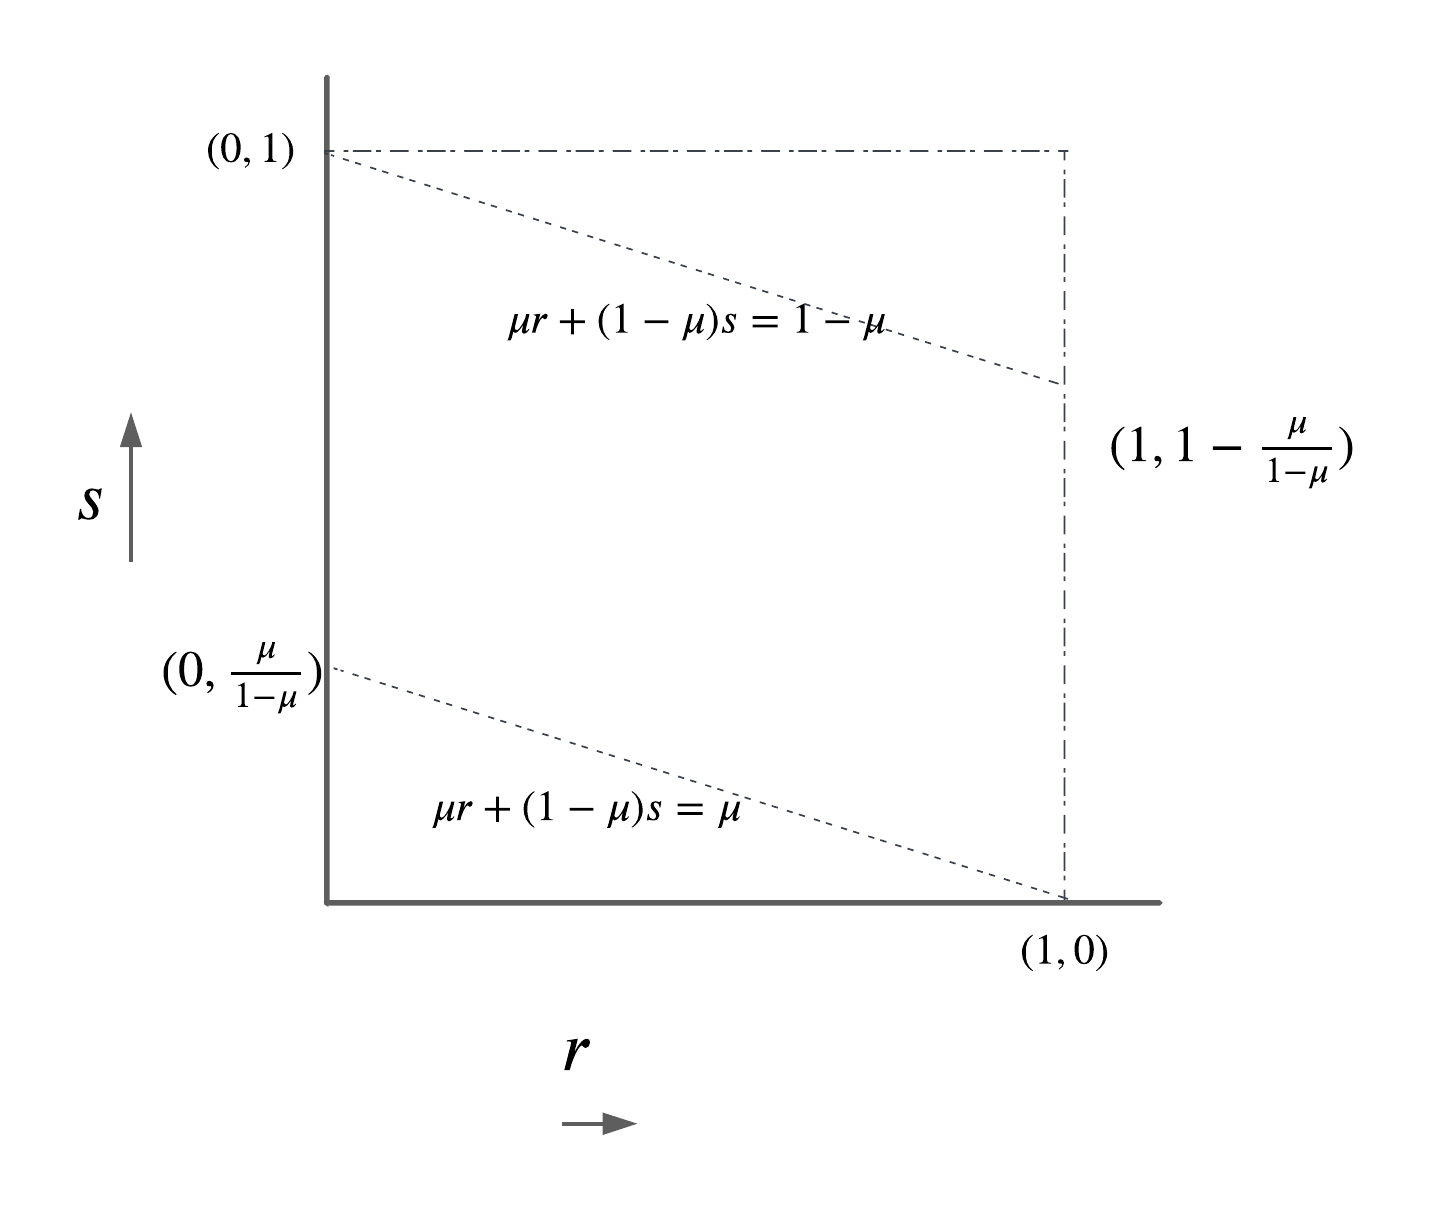
\includegraphics[width=4in]{figures/integral_calculation}
\par\end{centering}
\caption{\label{fig:integral_boundaries}Integration over $r,s$ split by boundaries
$\mu r+(1-\mu)s=\mu$ and $\mu r+(1-\mu)s=1-\mu$}
\end{figure}

\end{appendices}
\end{document}
